\documentclass[11pt,compress,t,notes=noshow, aspectratio=169, xcolor=table]{beamer}

\usepackage{../../style/lmu-lecture}
% Defines macros and environments
% This file is included in slides and exercises

% Rarely used fontstyle for R packages, used only in 
% - forests/slides-forests-benchmark.tex
% - exercises/single-exercises/methods_l_1.Rnw
% - slides/cart/attic/slides_extra_trees.Rnw
\newcommand{\pkg}[1]{{\fontseries{b}\selectfont #1}}

% Spacing helpers, used often (mostly in exercises for \dlz)
\newcommand{\lz}{\vspace{0.5cm}} % vertical space (used often in slides)
\newcommand{\dlz}{\vspace{1cm}}  % double vertical space (used often in exercises, never in slides)
\newcommand{\oneliner}[1] % Oneliner for important statements, used e.g. in iml, algods
{\begin{block}{}\begin{center}\begin{Large}#1\end{Large}\end{center}\end{block}}

% Don't know if this is used or needed, remove?
% textcolor that works in mathmode
% https://tex.stackexchange.com/a/261480
% Used e.g. in forests/slides-forests-bagging.tex
% [...] \textcolor{blue}{\tfrac{1}{M}\sum^M_{m} [...]
% \makeatletter
% \renewcommand*{\@textcolor}[3]{%
%   \protect\leavevmode
%   \begingroup
%     \color#1{#2}#3%
%   \endgroup
% }
% \makeatother


\title{Interpretable Machine Learning}
% \author{LMU}
%\institute{\href{https://compstat-lmu.github.io/lecture_iml/}{compstat-lmu.github.io/lecture\_iml}}
\date{}

\begin{document}

% TODO
\newcommand{\titlefigure}{figure_man/molnar-shapplot.png}
\newcommand{\learninggoals}{
\item Get an intuition of additive feature attributions
\item Understand the concept of Kernel SHAP
\item Ability to interpret SHAP plots
\item Global SHAP methods
}

\lecturechapter{SHAP (SHapley Additive exPlanation) Values}
\lecture{Interpretable Machine Learning}


\begin{vbframe}{Shapley Values in ML - A short Recap}
  
  \textbf{Question:} How much does a feature $j$ contribute to the prediction of a single observation. \\
  \textbf{Theory:} Shapley Game Theory \\
  \textbf{Solution:} 
  \begin{itemize}
    \item Compare feature Coalition $S$ with $\Scupj$ 
    \item Iterate over possible coaltions to achive the marginal contibution of feature j to sample $\xv$. 
\end{itemize}

     $$ \phi_j  = \frac{1}{p!} \sum_{\Scupj} \underbrace{\fh_{\Scupj}(\xv_{\Scupj}) - \fh_{S}(\xv_{S})}_{\text{marginal contribution of feature $j$}} $$

\textbf{Remember:}

\begin{itemize}
    \item $\fh$ is an arbitrary prediction algorithm
    \item p denotes the amount of coalitions in S
    \item Non-existent features in the Coalition are replaced by randomly drawn states from the feature
\end{itemize}

\end{vbframe}

\begin{vbframe}{Idea}

\begin{itemize}
    \item Give intro to the example instance $\xv$
    \item What if we could quantify the contribution of each feature to achieve $\fh(\xv)$
    \item this would leave to an additional model like a linreg
\end{itemize}

\begin{tikzpicture}
\node[draw,rectangle,minimum width=7cm,minimum height=1.2cm] (n1) {(1)};
\node[draw,rectangle,minimum width=4cm,minimum height=0.9cm,above=0 of n1.north west,anchor=south west,node distance=0] (n21) {(2,1)};
\node[draw,rectangle,minimum width=3cm,minimum height=0.9cm,right=0 of n21.east,anchor=west,node distance=0] (n22) {(2,2)};
\end{tikzpicture}

\end{vbframe}

\begin{vbframe}{Motivation}
Find an additive combination that explains the prediction of an instance $\xv$ by computing the contribution of each feature to the prediction.

\begin{exampleblock}{}
\[
g\left(\tikzmark{z} z^{\prime}\right)=
\tikzmark{ph0}\phi_{0}+\sum_{j=1}^{M}
\tikzmark{phj} \phi_{j} z_{j}^{\prime}
\]
\begin{tikzpicture}[
  remember picture,
  overlay,
  expl/.style={draw=blue,fill=white,rounded corners,text width=3cm},
  arrow/.style={blue,ultra thick,->,>=latex}
]
\node<1-3>[expl] 
  (zex) 
  at (2,1.5cm)
  {$z^{\prime}$:\textbf{Coalition} \\ simplified features};
\node<2-3>[expl] 
  (ph0ex) 
  at (5,-.5cm)
  {$\phi_0$: \textbf{Null Output} \\ Average Model Baseline};
\node<3>[expl] 
  (phjex) 
  at (12,0cm)
  {$\phi_j$: \textbf{Attribution} \\ How much does feature $j$ change the output};

\draw<1-3>[arrow]
  (zex.east) to[out=180,in=90] ([xshift= 1ex, yshift=1.5ex]{pic cs:z});  
\draw<2-3>[arrow]
  (ph0ex.east) to[out=180,in=270] ([xshift= 1ex, yshift=-0.5ex]{pic cs:ph0});  
\draw<3>[arrow]
  (phjex.west) to[out=90,in=270] ([xshift= 1ex, yshift=-0.5ex]{pic cs:phj});  
\node<4>[expl] 
  (phjsh) 
  at (10.5,2cm)
  {$\phi_j$: \textbf{Sahpley Values}};
\draw<4>[arrow]
  (phjsh.west) to[out=90,in=90] ([xshift= 1ex, yshift=1ex]{pic cs:phj}); 
\draw<4> [
    thick,
    decoration={
        brace,
        mirror,
        raise=0.5cm
    },
    decorate
] (7,0.7) -- (9.5,0.7)
node[pos=0.5,below=15pt,black]{\textbf{Additive Feature Attribution}};
\end{tikzpicture}
\end{exampleblock}

\vspace{1cm}
\textbf{Notice}
\begin{itemize}
    \item Looks like a linear model?
    \item Let $z^{\prime} \in \{0, 1\}^M$ be the coalition vector, indicating if feature $j$ contributes to the prediction.
    \item Let $h_{x}$ represent a function that maps 1’s to the corresponding value from the instance x that we want to explain: $h_{x}\left(z^{\prime}\right)=z \text { where } h_{x}:\{0,1\}^{M} \rightarrow \mathbb{R}^{p}$. $h_{x}$ connects our coalition vector to the underlying data.
\end{itemize}

\end{vbframe}


\begin{vbframe}{Kernel SHAP - In 5 Steps}

\textbf{Definition:} A kernel based, model agnostic alternative for Shapley Values using local surrogate models.\\
\vspace{1cm}
\begin{enumerate}
    \item Sample Coalitions 
    \begin{onlyenv}<1>
    $$z_{k}^{\prime} \in\{0,1\}^{M}, \quad k \in\{1, \ldots, K\}$$
    \end{onlyenv}
    
    \item Transfer Coalitions into feature space \& get predictions by applying the model
    
    \begin{onlyenv}<2>
    $$\hat{f}: \hat{f}\left(h_{x}\left(z_{k}^{\prime}\right)\right)$$
    \end{onlyenv}
    
    \item Compute weights through Kernel
    \begin{onlyenv}<3>
    $$\pi_{x}\left(z^{\prime}\right)=\frac{(M-1)}{\left(\begin{array}{c} M \\\left|z^{\prime}\right|\end{array}\right)\left|z^{\prime}\right|\left(M-\left|z^{\prime}\right|\right)}$$
    \end{onlyenv}
    
    \item Fit a weighted linear model by optimizing Loss
    \begin{onlyenv}<4>
    $$L\left(\hat{f}, g, \pi_{x}\right)=\sum_{z^{\prime} \in Z}\left[\hat{f}\left(h_{x}\left(z^{\prime}\right)\right)-g\left(z^{\prime}\right)\right]^{2} \pi_{x}\left(z^{\prime}\right)$$
    \end{onlyenv}

    \item Return shapley values
    \begin{onlyenv}<5>
    $$(\phi_1, \ldots, \phi_M)$$
    \end{onlyenv}
    
    
\end{enumerate}

\end{vbframe}

\begin{vbframe}{Form and evaluate Coalitions}

\begin{figure}
    \centering
    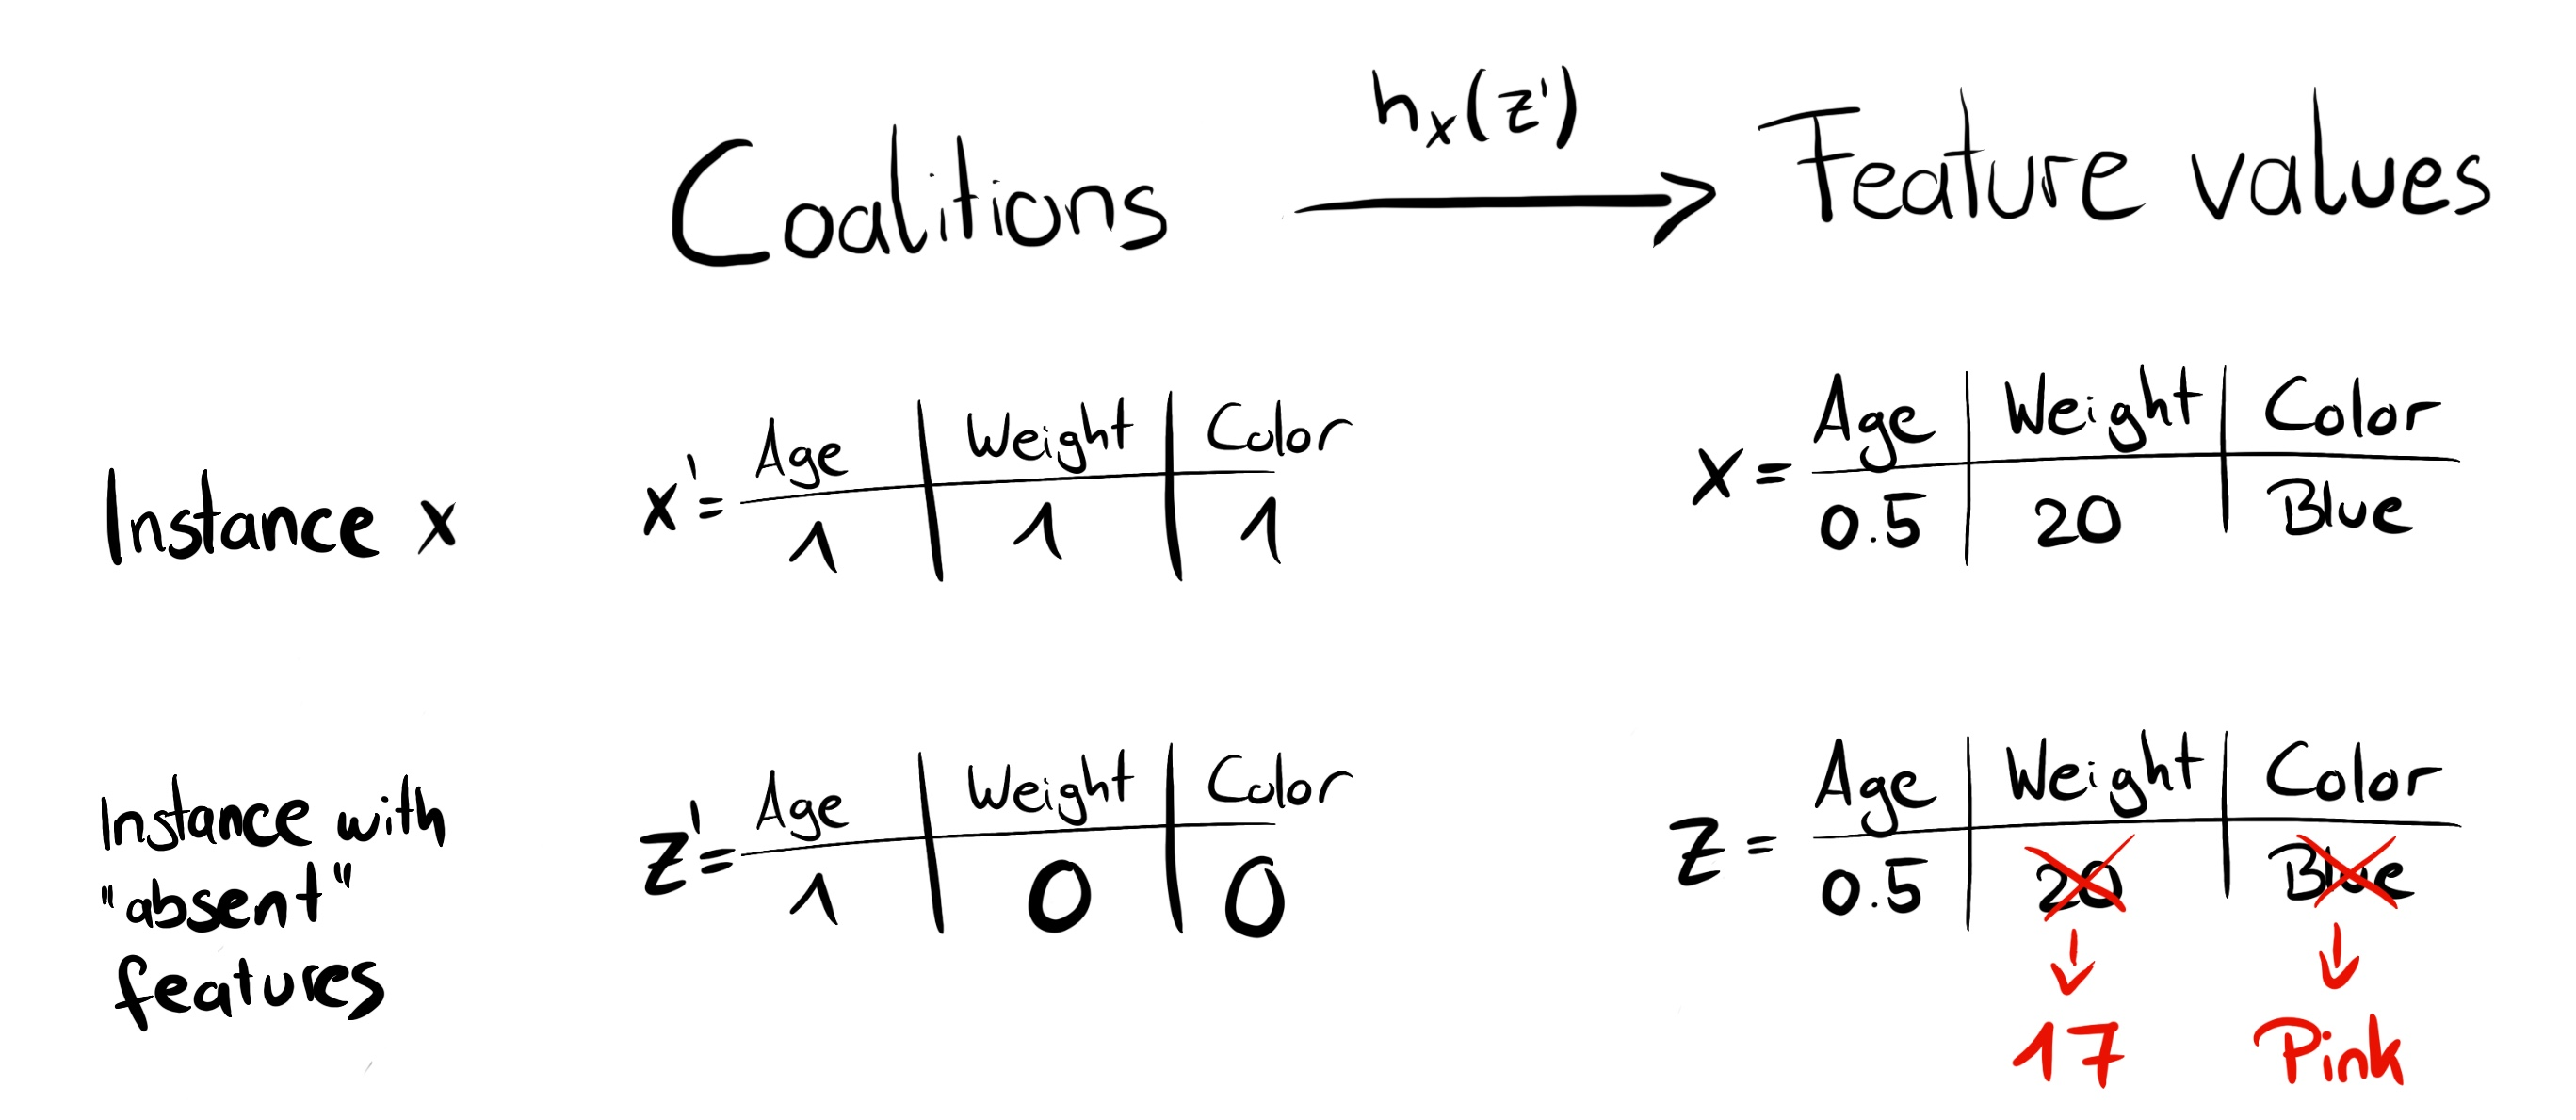
\includegraphics{figure_man/molnar-simplified-features.jpg}
\end{figure}

 \end{vbframe}
 
\begin{vbframe}{The Kernel}
\textbf{Intuition}: We learn most about individual features if we can study their effects in isolation or at maximal interaction:\\
Small coalitions (few 1’s) and large coalitions (i.e. many 1’s) get the largest weights
\begin{itemize}
    \item If a coalition consists of a single feature, we can learn about this feature’s isolated main effect on the prediction
    \item If a coalition consists of all but one feature, we can learn about this feature’s total effect (main effect plus feature interactions)
    \item If a coalition consists of half the features, we learn little about an individual feature’s contribution, as there are many possible coalitions with half of the features
\end{itemize}

\begin{onlyenv}<2>
\begin{exampleblock}{Definition}
\[
\tikzmark{pi}\pi_{x}\left(z^{\prime}\right)=\frac{(
\tikzmark{M}M-1)}{\left(\begin{array}{c} M \\\left|z^{\prime}\right|\end{array}\right)\left|
\tikzmark{z}z^{\prime}\right|\left(M-\left|z^{\prime}\right|\right)}
\]
\begin{tikzpicture}[
  remember picture,
  overlay,
  expl/.style={draw=blue,fill=white,rounded corners,text width=3cm},
  arrow/.style={blue,ultra thick,->,>=latex}
]
\node[expl] 
  (piex) 
  at (0,1cm)
  {$\pi_x(\prime{z})$: kernel weight for coalition $\prime{z}$};
\node[expl] 
  (Mex) 
  at (6,1cm)
  {M: Amount of features in x};
\node[expl] 
  (zex) 
  at (3,-1cm)
  {$\mid\prime{z}\mid$: coalition size / sum of 1s in $\prime{z}$};
\draw[arrow]
  (piex.west) to[out=180,in=135] ([xshift= 0.5ex, yshift=2ex]{pic cs:pi}); 
\draw[arrow]
  (Mex.west) to[out=180,in=135] ([xshift= 0.5ex, yshift=2ex]{pic cs:M}); 
\draw[arrow]
  (zex.north) to[out=180,in=135] ([xshift= 0.5ex, yshift=2ex]{pic cs:z}); 
\end{tikzpicture}
\end{exampleblock}
\end{onlyenv}




\begin{onlyenv}<2>
\textbf{Limited Budget $K$}: Can we be a bit smarter about the sampling of coalitions, than just randomly drawing?
\begin{itemize}
    \item The smallest and largest coalitions take up most of the weight. We get better Shapley value estimates by using some of the sampling budget K to include these high-weight coalitions.
    \item We start with all possible coalitions with 1 and M-1 features, which makes 2 times M coalitions in total. When we have enough budget left (current budget is K - 2M), we can include coalitions with 2 features and with M-2 features and so on.
    \item From the remaining coalition sizes, we sample with readjusted weights.
\end{itemize}
\end{onlyenv}
  

 \end{vbframe}
 
 \begin{vbframe}{Linear Model and Coefficients}

 \end{vbframe}
 
\begin{vbframe}{Example}

\begin{figure}
    \centering
    \includegraphics[width=0.7\columnwidth]{figure_man/molnar-shapplot.png}
\end{figure}

\end{vbframe}

\begin{vbframe}{Properties}

\textbf{Local Accuracy}
$$
f(x)=g\left(x^{\prime}\right)=\phi_{0}+\sum_{j=1}^{M} \phi_{j} x_{i}^{\prime}
$$
\begin{onlyenv}<1>
\textbf{Intution:} If the coalition includes all features ($x^{\prime}  \in \{1\}^M $), the attributions $\phi_j$ should sum up with the base line $\phi_0$ to the original model output for observation $f(\xv)$ \\
Local Accuracy corresponds to the \textbf{Axiom of Efficiency} in Shapley Game Theory 

\end{onlyenv}

\begin{onlyenv}<2->
\textbf{Missingness}
$$
x_{i}^{\prime}=0 \Longrightarrow \phi_{i}=0
$$
\end{onlyenv}

\begin{onlyenv}<2>
\textbf{Intution:}  A missing feature gets an attribution of zero
\end{onlyenv}

\begin{onlyenv}<3->
\textbf{Consistency} \\
\end{onlyenv}
\begin{onlyenv}<3>
$f_{x}\left(z^{\prime}\right)=f\left(h_{x}\left(z^{\prime}\right)\right) \text { and } z^{\prime}_{\backslash  i} \text{ denote setting } z_{i}^{\prime}=0$ . For any two
models $f$ and $f^{\prime}$, if
$$
f_{x}^{\prime}\left(z^{\prime}\right)-f_{x}^{\prime}\left(z^{\prime}_{\backslash i}\right) \geq f_{x}\left(z^{\prime}\right)-f_{x}\left(z^{\prime}_{\backslash i}\right)
$$
for all inputs $z^{\prime} \in \{0, 1\}^M$, then
$$
\phi_{i}\left(f^{\prime}, x\right) \geq \phi_{i}(f, x)
$$
\end{onlyenv}

\begin{onlyenv}<4->
$$
f_{x}^{\prime}\left(z^{\prime}\right)-f_{x}^{\prime}\left(z^{\prime}_{\backslash i}\right) \geq f_{x}\left(z^{\prime}\right)-f_{x}\left(z^{\prime} _{\backslash i}\right) \Longrightarrow \phi_{i}\left(f^{\prime}, x\right) \geq \phi_{i}(f, x)
$$

\textbf{Intution:} If a model changes so that the marginal contribution of a feature value increases or stays the same, the Shapley value also increases or stays the same\\ 
From Consistency the Shapley \textbf{Axioms of Linearity, Dummy and Symmetry} follow.
\end{onlyenv}


\end{vbframe}

\begin{vbframe}{Tree SHAP}

\end{vbframe}

 \begin{vbframe}{Global SHAP}
\textbf{Idea: }
If we run SHAP for every instance, we get a matrix of Shapley values. This matrix has one row per data instance and one column per feature. We can interpret the entire model by analyzing the Shapley values in this matrix.
\vspace{2cm}
$$
\Phi =
\begin{bmatrix}
    \phi_{11} & \phi_{12} & \phi_{13} & \dots  & \phi_{1M} \\
    \phi_{21} & \phi_{22} & \phi_{23} & \dots  & \phi_{2M} \\
    \vdots & \vdots & \vdots & \ddots & \vdots \\
    \phi_{n1} & \phi_{n2} & \phi_{n3} & \dots  & \phi_{nM} \\
\end{bmatrix}
$$

 \end{vbframe}

 \begin{vbframe}{Feature Importance}
 
\textbf{Idea:} Average the Shapley values of each feature over all instances. This corresponds to calculating column-wise averages in $\Phi$
$$
I_{j}=\frac{1}{n} \sum_{i=1}^{n}\left|\phi_{j}^{(i)}\right|
$$
\end{vbframe}
 
\begin{vbframe}{Summary Plot}
\end{vbframe} 

\begin{vbframe}{Dependence Plot}
\end{vbframe}

\begin{vbframe}{Discussion}
\begin{onlyenv}<1>
\textbf{Advantages}

Since SHAP computes Shapley values, all the advantages of Shapley values apply: SHAP has a solid theoretical foundation in game theory. The prediction is fairly distributed among the feature values. We get contrastive explanations that compare the prediction with the average prediction.

SHAP connects LIME and Shapley values. This is very useful to better understand both methods. It also helps to unify the field of interpretable machine learning.

SHAP has a fast implementation for tree-based models. I believe this was key to the popularity of SHAP, because the biggest barrier for adoption of Shapley values is the slow computation.

The fast computation makes it possible to compute the many Shapley values needed for the global model interpretations. The global interpretation methods include feature importance, feature dependence, interactions, clustering and summary plots. With SHAP, global interpretations are consistent with the local explanations, since the Shapley values are the “atomic unit” of the global interpretations. If you use LIME for local explanations and partial dependence plots plus permutation feature importance for global explanations, you lack a common foundation.
\end{onlyenv}

\begin{onlyenv}<2>
\textbf{Disadvantages}

KernelSHAP is slow. This makes KernelSHAP impractical to use when you want to compute Shapley values for many instances. Also all global SHAP methods such as SHAP feature importance require computing Shapley values for a lot of instances.

KernelSHAP ignores feature dependence. Most other permutation based interpretation methods have this problem. By replacing feature values with values from random instances, it is usually easier to randomly sample from the marginal distribution. However, if features are dependent, e.g. correlated, this leads to putting too much weight on unlikely data points. TreeSHAP solves this problem by explicitly modeling the conditional expected prediction.

TreeSHAP can produce unintuitive feature attributions. While TreeSHAP solves the problem of extrapolating to unlikely data points, it does so by changing the value function and therefore slightly changes the game. TreeSHAP changes the value function by relying on the conditional expected prediction. With the change in the value function, features that have no influence on the prediction can get a TreeSHAP value different from zero.

The disadvantages of Shapley values also apply to SHAP: Shapley values can be misinterpreted and access to data is needed to compute them for new data (except for TreeSHAP).

It is possible to create intentionally misleading interpretations with SHAP, which can hide biases 72. If you are the data scientist creating the explanations, this is not an actual problem (it would even be an advantage if you are the evil data scientist who wants to create misleading explanations). For the receivers of a SHAP explanation, it is a disadvantage: they cannot be sure about the truthfulness of the explanation.

\end{onlyenv}

\end{vbframe}

\endlecture
\end{document}
